\chapter{Formulario T-14: Plan de trabajo, EDT y carta Gantt}

Este formulario detalla lo que el Subdocumento 7 resume en sus secciones 7.1 y 7.3, conforme al Formulario T-14 de las Bases Administrativas y al Capítulo 7 del índice obligatorio de las Aclaraciones de la licitación. Contiene la estructura de descomposición del trabajo (EDT) completa; su diccionario, con el entregable, el criterio de aceptación, el responsable y el período de cada paquete; y la carta Gantt de los 56 meses del contrato. El método de estimación y programación, la ruta crítica y los frentes de trabajo se detallan en el Formulario T-15, y la implantación de cada etapa, en el Formulario T-18. La EDT termina en el paquete de trabajo; la descomposición de cada paquete en actividades de 8 a 80 horas hombre que caben en una quincena, con sus fechas, está en el Formulario T-15, sección 6. La EDT termina en el paquete de trabajo; la descomposición de cada paquete en actividades de 8 a 80 horas hombre que caben en una quincena está en el Formulario T-15, sección 6.

\section{Estructura de descomposición del trabajo}

La EDT descompone el 100 \% del alcance de la Etapa 1, la Etapa 2 y la Operación (Bases Administrativas, Art. 15°) en nueve fases, 49 cuentas de control y 222 paquetes de trabajo. Las fases 1 a 4 son las del proceso de desarrollo declarado en el Capítulo 6 (Inicio, Elaboración, Construcción y Transición) y se recorren una vez por etapa. Las fases 5 a 9 agrupan el trabajo que no es desarrollo de software. Cada paquete es la hoja de su rama, tiene un único responsable y produce un entregable verificable. En la cuenta 3.10, cada innovación agrupa sus paquetes en un cuarto nivel. La Tabla \ref{tab:T14-1} resume el tamaño de cada fase.

\parte{tablas/tab_T14_1}

La construcción concentra 79 de los 222 paquetes, y las fases que no son software (5 a 7) suman 50. Ninguna cuenta de control tiene un solo paquete. La estructura completa es la siguiente, con la raíz «Plataforma logística de Distribuidora Puelche» y sus nueve fases en el primer nivel.

\begin{itemize}
\item \textbf{1. Inicio}

\item 1.1 Definición inicial del proyecto

\item 1.1.1 Acta de constitución del proyecto, firmada con la Contraparte Técnica

\item 1.1.2 Documento de validación con el CLIENTE de los problemas y metas del proyecto

\item 1.1.3 Acta de confirmación con el CLIENTE de la fecha de inicio, la evidencia para el proveedor de lácteos, las ventanas de paso a producción y el acuse tributario

\item 1.2 Alcance del proyecto

\item 1.2.1 Documento de especificación de requerimientos y línea base de alcance de la Etapa 1 (H1)

\item 1.2.2 Documento de reglas de ruteo capturadas al planificador de rutas

\item 1.2.3 Documento de especificación de las interfaces sin documentación del ERP, del WMS de 2013 y de la telemetría del tercero

\item 1.2.4 Matriz de trazabilidad: requerimiento, módulo, paquete y prueba (H1)

\item 1.2.5 Documento de línea base de alcance de la Etapa 2: canal moderno y costo de servir (H8)

\item 1.3 Planificación del proyecto

\item 1.3.1 Plan para la dirección del proyecto, con el calendario de congelamientos de septiembre, diciembre y el cierre mensual

\item 1.3.2 EDT y diccionario de la EDT (línea base del alcance)

\item 1.3.3 Carta Gantt de 56 meses con los hitos H1 a H12 y la ruta crítica

\item 1.3.4 Documento de nivelación de recursos y frentes del solapamiento de los meses 13 a 15 y 19 a 20

\item 1.3.5 Reunión semanal de seguimiento con su informe semanal

\item 1.4 Gestión de interesados y comunicaciones

\item 1.4.1 Registro de interesados con su influencia, interés y estrategia

\item 1.4.2 Plan de comunicaciones con calendario y canales por grupo de interés

\item 1.4.3 Registro de solicitudes de cambio con análisis de impacto

\item 1.5 Gestión de calidad

\item 1.5.1 Plan de calidad y plan de pruebas

\item 1.5.2 Puertas de calidad automáticas en la cadena de integración (cobertura mínima del 80 \%)

\item 1.6 Gestión de riesgos

\item 1.6.1 Plan de riesgos y registro inicial de riesgos según ISO 31000

\item 1.6.2 Registro de riesgos revisado en cada Comité de Proyecto

\item 1.7 Plan de Reversibilidad

\item 1.7.1 Plan de Reversibilidad inicial (primeros 90 días)

\item 1.7.2 Primera actualización anual del Plan de Reversibilidad durante la implementación

\item 1.8 Gobierno y control del proyecto

\item 1.8.1 Oficina de gestión del proyecto con metodología basada en el PMBOK

\item 1.8.2 Actas del Comité Ejecutivo mensual, con la aprobación de los cambios de alcance

\item 1.8.3 Actas del Comité de Proyecto quincenal

\item 1.8.4 Actas del Comité de Arquitectura mensual

\item 1.8.5 Actas del Comité de Operación mensual, desde el mes 13

\item 1.8.6 Informe mensual de avance con valor ganado

\item 1.8.7 Tablero de estado del proyecto disponible para el CLIENTE

\item 1.8.8 Espacio colaborativo con la documentación, los entregables, las actas, los riesgos y los cambios

\item 1.9 Cumplimiento normativo y contractual

\item 1.9.1 Matriz de cumplimiento normativo por obligación legal, con su control y su evidencia

\item 1.9.2 Acuerdo de tratamiento de datos personales con el CLIENTE

\item 1.9.3 Registro de actividades de tratamiento y evaluación de impacto en protección de datos

\item 1.9.4 Certificación ISO/IEC 27001 vigente y entrega anual de los informes de certificación

\item 1.9.5 Garantía de fiel cumplimiento, seguros y certificados laborales vigentes durante el contrato

\item \textbf{2. Elaboración}

\item 2.1 Arquitectura de la solución

\item 2.1.1 Documento de arquitectura lógica: capas, módulos M1 a M12 e interfaces

\item 2.1.2 Documento de arquitectura física híbrida: nube, centros de distribución y plataformas de cross-docking

\item 2.1.3 Modelo de datos y diccionario de datos, con la trazabilidad por lote

\item 2.1.4 Documento de diseño detallado de M11 y del intercambio con las cadenas

\item 2.2 Diseño de la seguridad

\item 2.2.1 Plan de seguridad de la información

\item 2.2.2 Modelado de amenazas por componente y por integración externa, actualizado ante cada cambio

\item 2.2.3 Plan de respuesta a incidentes de seguridad, con aviso al CLIENTE en dos horas

\item 2.2.4 Matriz de clasificación de la información y matriz de controles

\item 2.3 Diseño de la sala técnica y de los racks

\item 2.3.1 Plano de la sala técnica de Talca, con su cálculo eléctrico y térmico

\item 2.3.2 Plano de distribución de los racks R01 de servidores y R02 de comunicaciones

\item 2.3.3 Plano de los gabinetes de borde de Concepción y de las plataformas de cross-docking

\item 2.4 Validación de diseños

\item 2.4.1 Acta de aprobación de la arquitectura, el plan de seguridad y el modelo de datos (H2)

\item 2.4.2 Acta de aprobación del diseño detallado de la Etapa 2 (H8)

\item 2.5 Continuidad del negocio

\item 2.5.1 Plan de continuidad del negocio según ISO 22301, con análisis de impacto y procedimientos manuales

\item 2.5.2 Plan de continuidad TIC según ISO/IEC 27031 y plan de recuperación ante desastres

\item 2.6 Experiencia de usuario

\item 2.6.1 Investigación con preparadores, preventistas, conductores y almaceneros

\item 2.6.2 Prototipos y pruebas de usabilidad con participantes del CLIENTE

\item 2.6.3 Indicadores de usabilidad comprometidos por transacción crítica

\item \textbf{3. Construcción}

\item 3.1 Ambientes y cadena de desarrollo

\item 3.1.1 Ambientes de Desarrollo y QA en la nube (H3)

\item 3.1.2 Ambientes de Preproducción y Producción en la nube (H3)

\item 3.1.3 Ambiente de recuperación ante desastres en la región secundaria (H3)

\item 3.1.4 Cadena de integración y entrega continua, e infraestructura como código

\item 3.1.5 Observabilidad de los doce módulos y de los sitios, con tableros para el CLIENTE (H3)

\item 3.2 Servicios de nube de la plataforma

\item 3.2.1 Servicio de nube para la aplicación y los portales

\item 3.2.2 Servicio de nube de base de datos, caché y mensajería

\item 3.2.3 Servicio de nube de ingesta de IoT, telemetría cruda y plataforma analítica

\item 3.2.4 Servicio de nube de respaldo inmutable y réplica entre regiones

\item 3.2.5 Servicio de nube de seguridad y gobierno, y detección en endpoints

\item 3.2.6 Servicio de gestión de dispositivos móviles

\item 3.3 Base compartida

\item 3.3.1 Identidad y control de acceso, incluidos los conductores externos que rotan sin aviso

\item 3.3.2 Integración con el ERP como único emisor de la guía de despacho (INT-06 e INT-07)

\item 3.3.3 Convivencia con el WMS de 2013 durante el reemplazo

\item 3.3.4 Integración con la telemetría de los 42 camiones propios (INT-15)

\item 3.3.5 Registro auditable de stock, lotes y cobros

\item 3.3.6 Operación sin conexión: 14 horas en terreno y 24 horas en el CD

\item 3.4 Módulos de la Etapa 1

\item 3.4.1 Recepción de mercadería con captura de lote y vencimiento (M1 Recepción)

\item 3.4.2 Inventario por ubicación y lote, con FEFO y conteo cíclico (M2 Inventario)

\item 3.4.3 Preparación de pedidos en el turno de noche y en la cámara de congelado (M5 Preparación)

\item 3.4.4 Cadena de frío, retención de lotes y retiro sanitario (M9 Calidad y trazabilidad)

\item 3.4.5 Ingesta de temperatura y posición de la flota (M12 Telemetría)

\item 3.4.6 Aplicación móvil de preventa sin conexión, con stock y crédito (M3 Preventa)

\item 3.4.7 Planificación de rutas corregible por el planificador (M4 Rutas)

\item 3.4.8 Aplicación móvil de reparto con prueba de entrega digital (M6 Reparto)

\item 3.4.9 Devoluciones en terreno y control de envases (M8 Devoluciones y envases)

\item 3.4.10 Cobro en ruta, rendición y conciliación (M7 Cobranza y rendición)

\item 3.4.11 Indicadores operacionales y OTIF diario (M10 Analítica)

\item 3.5 Módulos de la Etapa 2

\item 3.5.1 Pedido electrónico y aviso de despacho para las cadenas, y portal de proveedores (M11 Canal moderno)

\item 3.5.2 Portal web de clientes: cuenta, saldo, entregas y documentos

\item 3.5.3 Portal web de transportistas: rutas asignadas del día siguiente

\item 3.5.4 Costo de servir por cliente y por entrega (M10 Analítica)

\item 3.6 Integraciones externas

\item 3.6.1 Intercambio de lote y trazabilidad con los proveedores

\item 3.6.2 Integración con la pasarela de pago para el cobro con tarjeta (INT-09)

\item 3.6.3 Integración con el servicio de mapas y geocodificación (INT-10)

\item 3.6.4 Integración con el servicio de avisos al cliente (INT-11)

\item 3.6.5 Intercambio electrónico con la principal cadena, con sus pruebas aprobadas (INT-08)

\item 3.6.6 Incorporación de las demás cadenas al intercambio electrónico (INT-08)

\item 3.7 Migración de datos

\item 3.7.1 Informe de perfilamiento y datos saneados

\item 3.7.2 Datos maestros cargados: 8.400 SKU, clientes e instalaciones

\item 3.7.3 Saldos migrados desde el WMS de Talca

\item 3.7.4 Saldos cargados en Concepción desde el conteo físico

\item 3.7.5 Acta de conciliación y corte fuera de las ventanas de congelamiento

\item 3.8 Pruebas de la Etapa 1

\item 3.8.1 Pruebas de integración, regresión e idempotencia en QA (H4)

\item 3.8.2 Pruebas de aceptación y de accesibilidad con preventistas, conductores y bodega

\item 3.8.3 Pruebas del perfil operacional: sin señal, sin enlace y a −22 °C con guantes

\item 3.8.4 Pruebas de carga con el peak de septiembre y de resiliencia

\item 3.8.5 Prueba de recuperación ante desastres con conmutación real

\item 3.8.6 Prueba de seguridad ofensiva de la Etapa 1, por un tercero independiente

\item 3.8.7 Acta de certificación de la Etapa 1 (H5)

\item 3.8.8 Demostración en Preproducción del despliegue sin interrupción de la Etapa 1

\item 3.9 Pruebas de la Etapa 2

\item 3.9.1 Pruebas de integración y regresión sin afectar la Etapa 1 en producción (H9)

\item 3.9.2 Pruebas de aceptación y de accesibilidad con cadenas, transportistas, Comercial y Finanzas

\item 3.9.3 Pruebas de carga con ambas etapas activas y de resiliencia

\item 3.9.4 Prueba de recuperación ante desastres con ambas etapas

\item 3.9.5 Prueba de seguridad ofensiva de la Etapa 2, por un tercero independiente

\item 3.9.6 Acta de certificación de la Etapa 2 y cierre del desarrollo (H10)

\item 3.9.7 Demostración en Preproducción del despliegue sin interrupción de la Etapa 2

\item 3.10 Innovaciones

\item 3.10.1 Innovación 1: seguimiento de vencimiento posentrega en el local

\item 3.10.1.1 Documento de catálogo de acciones y protocolo del piloto (INN-01.P1)

\item 3.10.1.2 Estimador de saldo y ritmo de reposición (INN-01.P2)

\item 3.10.1.3 Función de lista sin conexión en la aplicación de preventa (INN-01.P3)

\item 3.10.1.4 Informe del piloto en marcha blanca y habilitación (INN-01.P4)

\item 3.10.2 Innovación 2: reproducción de incidentes de terreno

\item 3.10.2.1 Informe de medición inicial y contrato de evidencia (INN-02.P1)

\item 3.10.2.2 Circuito mínimo de reproducción en la preventa (INN-02.P2)

\item 3.10.2.3 Captura de evidencia en las aplicaciones de preventa, preparación y reparto (INN-02.P3)

\item 3.10.2.4 Informe de validación comparada durante la implementación (INN-02.P4, primera parte)

\item 3.10.3 Innovación 3: vida útil remanente por historia térmica del lote

\item 3.10.3.1 Documento de familias priorizadas y parámetros aprobados (INN-03.P1)

\item 3.10.3.2 Asociación lote–sensor en el borde y en el camión (INN-03.P2)

\item 3.10.3.3 Vista en M9 y orden de salida sugerido (INN-03.P3)

\item 3.10.3.4 Informe de validación en marcha blanca con Calidad (INN-03.P4)

\item 3.10.4 Innovación 5: hoja de negocio del almacenero

\item 3.10.4.1 Prototipo e informe de la prueba de comprensión (INN-05.P1)

\item 3.10.4.2 Evaluación de privacidad y diseño de la impresión en cabina (INN-05.P2)

\item 3.10.4.3 Cálculo y bloques 1 a 3 de la hoja de negocio (INN-05.P3)

\item 3.10.4.4 Hoja certificada, en marcha blanca y en producción (INN-05.P4, primera parte)

\item 3.11 Documentación técnica

\item 3.11.1 Documentación técnica, funcional, de arquitectura, de operación y de seguridad

\item 3.11.2 Base de conocimiento de incidentes y decisiones de diseño

\item 3.11.3 Estándares de codificación y documentación de interfaces en OpenAPI y AsyncAPI

\item 3.11.4 Inventario de componentes (SBOM) con sus licencias de código abierto

\item 3.11.5 Depósito del código fuente en el repositorio del CLIENTE en cada liberación

\item \textbf{4. Transición}

\item 4.1 Plan de implantación

\item 4.1.1 Plan de olas de la Etapa 1 por sitio y zona: Talca, Concepción y plataformas de cross-docking

\item 4.1.2 Procedimiento de reversión de la Etapa 1 antes de las 05:30, con versión operativa local y DTE emitidos por el ERP

\item 4.1.3 Plan de implantación y reversión de la Etapa 2 fuera de la ventana de 05:30 a 07:00

\item 4.2 Marcha blanca y producción de la Etapa 1

\item 4.2.1 Marcha blanca de la Etapa 1 con conciliación diaria (H6)

\item 4.2.2 Estabilización de la Etapa 1 en el turno de noche y acompañamiento en ruta

\item 4.2.3 Acta de paso a producción y cierre de la Etapa 1 (H7)

\item 4.3 Marcha blanca y producción de la Etapa 2

\item 4.3.1 Marcha blanca de la Etapa 2 en convivencia con la Etapa 1 y fuente única de datos (H11)

\item 4.3.2 Estabilización de la Etapa 2 con Comercial, Finanzas, cadenas y transportistas

\item 4.3.3 Acta de paso a producción y aceptación final de la implementación (H12)

\item 4.3.4 Garantía de correcto funcionamiento constituida, condición de la aceptación final (H12)

\item \textbf{5. Adquisiciones y contrataciones}

\item 5.1 Hardware e infraestructura

\item 5.1.1 Especificación de compra del equipamiento de terreno para el CLIENTE

\item 5.1.2 Especificación y compra de la sala técnica, los racks, los servidores y los gabinetes de borde

\item 5.1.3 Actas de recepción técnica del equipamiento de terreno comprado por el CLIENTE y de la infraestructura provista por LafroX

\item 5.2 Servicios de nube y licencias

\item 5.2.1 Contrato de los servicios de AWS

\item 5.2.2 Suscripción del servicio de gestión de dispositivos y de detección en endpoints

\item 5.2.3 Licencias de software de terceros constituidas a nombre del CLIENTE

\item 5.3 Enlaces de comunicaciones

\item 5.3.1 Contrato de fibra óptica de los CD de Talca y Concepción

\item 5.3.2 Contrato de planes LTE con dos proveedores (ocho planes)

\item 5.3.3 Contrato de Starlink para los cinco sitios: Talca, Concepción y las tres plataformas de cross-docking

\item 5.4 Acuerdos con terceros

\item 5.4.1 Acuerdos operacionales firmados con los diez transportistas

\item 5.4.2 Acta de acuerdo con el sindicato sobre terminales, GPS y cámaras

\item 5.4.3 Fórmula aprobada del tramo variable: reglas de atribución, canasta e índices (INN-04.P1)

\item 5.4.4 Contrato de custodia de fuentes con un tercero independiente

\item \textbf{6. Infraestructura física y sitios}

\item 6.1 Adecuación de la sala técnica de Talca

\item 6.1.1 Coordinación de la obra civil de separación, a cargo del CLIENTE (RT-06.06), y piso técnico de la sala

\item 6.1.2 Hardware de energía instalado: UPS modular N+1, generador con 24 horas de autonomía, transferencia automática y PDU A/B

\item 6.1.3 Hardware de climatización de precisión N+1 instalado

\item 6.1.4 Hardware de detección temprana de incendio y extinción por agente limpio instalado

\item 6.1.5 Acta de recepción técnica de la sala

\item 6.2 Cableado estructurado

\item 6.2.1 Cableado de cobre Cat6A y fibra OM4 tendido, con dos ductos de ingreso independientes

\item 6.2.2 Certificación de enlaces, etiquetado y planos as-built

\item 6.2.3 Gabinetes de piso y switches de acceso instalados en las bodegas de Talca y Concepción

\item 6.3 Montaje de racks y gabinetes

\item 6.3.1 Rack R01 de servidores montado: clúster de tres nodos, respaldo local, consola KVM y traslado del servidor del ERP del CLIENTE a U25–U26, con respaldo completo verificado, en ventana dominical después del H3 y antes de la marcha blanca de Talca, sin cambios de software

\item 6.3.2 Rack R02 de comunicaciones montado: firewalls, switches de núcleo y de gestión, y distribución de fibra

\item 6.3.3 Gabinete de borde de Concepción montado: servidores activo y en espera, firewalls, switches, UPS, climatización y monitoreo, con toma del servicio por el de espera si falla el activo

\item 6.3.4 Gabinetes de borde montados en Curicó, Chillán y Los Ángeles, con dos mini-PC (activo y en espera) por plataforma

\item 6.4 Sistemas de seguridad física

\item 6.4.1 Hardware de control de acceso biométrico y esclusa instalado

\item 6.4.2 Hardware de videovigilancia instalado

\item 6.4.3 Recinto de custodia de respaldos habilitado

\item 6.5 Equipamiento de campo

\item 6.5.1 Terminales de preventa, reparto y bodega configurados y enrolados

\item 6.5.2 Terminales de pago configurados, uno por camión

\item 6.5.3 Sensores de cámara y gateways IoT instalados en Talca y Concepción

\item 6.5.4 Termógrafos instalados en los 28 camiones con frío (propios y de transportistas)

\item 6.5.5 Impresoras de cabina instaladas

\item 6.5.6 Impresoras de andén y balanzas de recepción instaladas

\item 6.6 Configuración de la infraestructura de los sitios

\item 6.6.1 Software de base instalado en los sitios: virtualización, contenedores, PostgreSQL, RabbitMQ y Keycloak

\item 6.6.2 Enlaces de fibra, LTE y Starlink habilitados, con conmutación al respaldo

\item 6.6.3 Borde de los CD en servicio, con la prueba de autonomía de 24 horas aprobada

\item \textbf{7. Capacitación y gestión del cambio}

\item 7.1 Capacitación por roles

\item 7.1.1 Plan de capacitación por perfil: usuarios finales, avanzados, administradores, equipo técnico y soporte

\item 7.1.2 Programa de capacitación continua del turno de noche por la rotación del 38 \%

\item 7.1.3 Procedimiento de incorporación de los conductores de los transportistas en el andén

\item 7.1.4 Traspaso al equipo de TI de cuatro personas del CLIENTE

\item 7.1.5 Materiales de capacitación: manuales por perfil, guías rápidas, preguntas frecuentes y videos tutoriales

\item 7.1.6 Plataforma de autoformación en línea con registro de avance

\item 7.2 Gestión del cambio

\item 7.2.1 Acompañamiento del personal con 20 o 30 años en la compañía

\item 7.2.2 Gestión del cambio con las cadenas y los transportistas

\item 7.2.3 Diagnóstico del impacto organizacional por área y perfil, con agentes de cambio

\item 7.2.4 Procedimientos operativos afectados, rediseñados y documentados

\item 7.2.5 Medición de la adopción y plan de acción correctiva

\item 7.3 Evaluaciones y certificaciones

\item 7.3.1 Certificación de preventistas, conductores y preparadores (Etapa 1)

\item 7.3.2 Certificación de Comercial y Finanzas en costo de servir (Etapa 2)

\item \textbf{8. Operación y soporte (36 meses)}

\item 8.1 Servicios de operación

\item 8.1.1 Servicio de centro de operaciones 24\ensuremath{\times}7 y mesa de servicio durante los 36 meses de operación (04:00 a 22:00; 24\ensuremath{\times}7 en septiembre y diciembre)

\item 8.1.2 Servicio de gestión de incidentes, problemas y niveles de servicio del Art. 78° durante los 36 meses de operación

\item 8.1.3 Servicio de continuidad y pruebas semestrales de recuperación ante desastres durante los 36 meses de operación

\item 8.1.4 Actualizaciones anuales del Plan de Reversibilidad durante los 36 meses de operación

\item 8.1.5 Servicio de centro de operaciones de seguridad 24\ensuremath{\times}7 con SIEM durante los 36 meses de operación

\item 8.1.6 Pruebas mensuales de restauración de respaldos durante los 36 meses de operación

\item 8.2 Mantenimiento

\item 8.2.1 Mantenimiento correctivo y evolutivo del software durante los 36 meses de operación, con bolsa anual de horas y fuera de las ventanas de congelamiento

\item 8.2.2 Mantenimiento de ciberseguridad durante los 36 meses de operación: vulnerabilidades, intrusión anual e inyección de fallas

\item 8.2.3 Mantenimiento del hardware durante los 36 meses de operación: sala técnica, racks, gabinetes de borde y equipamiento de terreno

\item 8.2.4 Registro y reducción de la deuda técnica durante los 36 meses de operación

\item 8.2.5 Actualizaciones anuales de los componentes de base durante los 36 meses de operación

\item 8.2.6 Revisiones semestrales de las instalaciones eléctricas de la sala durante los 36 meses de operación

\item 8.2.7 Ciclo de vida del equipamiento durante los 36 meses de operación: reposición y disposición final

\item 8.3 Innovaciones en operación

\item 8.3.1 Innovación 2: mantenimiento de escenarios de regresión (INN-02.P4, segunda parte)

\item 8.3.2 Innovación 3: revisión semestral de parámetros durante los 36 meses de operación (INN-03.P5)

\item 8.3.3 Innovación 4: línea base y liquidaciones en sombra (INN-04.P2)

\item 8.3.4 Innovación 4: liquidación mensual del tramo variable, meses 24 a 56 (INN-04.P3)

\item 8.3.5 Innovación 5: despliegue gradual por rutas (INN-05.P4, segunda parte)

\item 8.3.6 Innovación 5: bloque 4 condicionado (INN-05.P5)

\item 8.4 Informes y obligaciones periódicas

\item 8.4.1 Gestión de la capacidad con proyección trimestral durante los 36 meses de operación

\item 8.4.2 Informes mensuales de consumo de nube (FinOps) durante los 36 meses de operación

\item 8.4.3 Estimaciones anuales de la huella de carbono de la operación

\item 8.4.4 Actualizaciones semestrales del depósito de custodia de fuentes durante los 36 meses de operación

\item 8.5 Capacitación y transferencia en operación

\item 8.5.1 Dos jornadas anuales de actualización y capacitación del personal nuevo durante los 36 meses de operación

\item 8.5.2 Mentoría al equipo técnico del CLIENTE durante los seis meses posteriores al mes 21

\item 8.5.3 Mantenimiento de la base de conocimiento durante los 36 meses de operación, con métricas de uso

\item \textbf{9. Cierre}

\item 9.1 Cierre de la implementación

\item 9.1.1 Entrega del código fuente, la infraestructura como código y los procedimientos de despliegue

\item 9.1.2 Informe de lecciones aprendidas y archivo de la implementación

\item 9.2 Salida al término del contrato

\item 9.2.1 Ejecución del Plan de Reversibilidad y acompañamiento de 90 días

\item 9.2.2 Certificado de devolución o eliminación de datos personales

\end{itemize}
La figura siguiente presenta la EDT completa en una sola vista panorámica. Por su densidad, se recomienda ampliarla en el PDF; el Subdocumento 7 contiene las láminas separadas por fase para consultar las cuentas de control y los paquetes con mayor legibilidad.

\begin{anexohorizontal}
\setlength{\textwidth}{\linewidth}
\thispagestyle{empty}
\begin{center}
  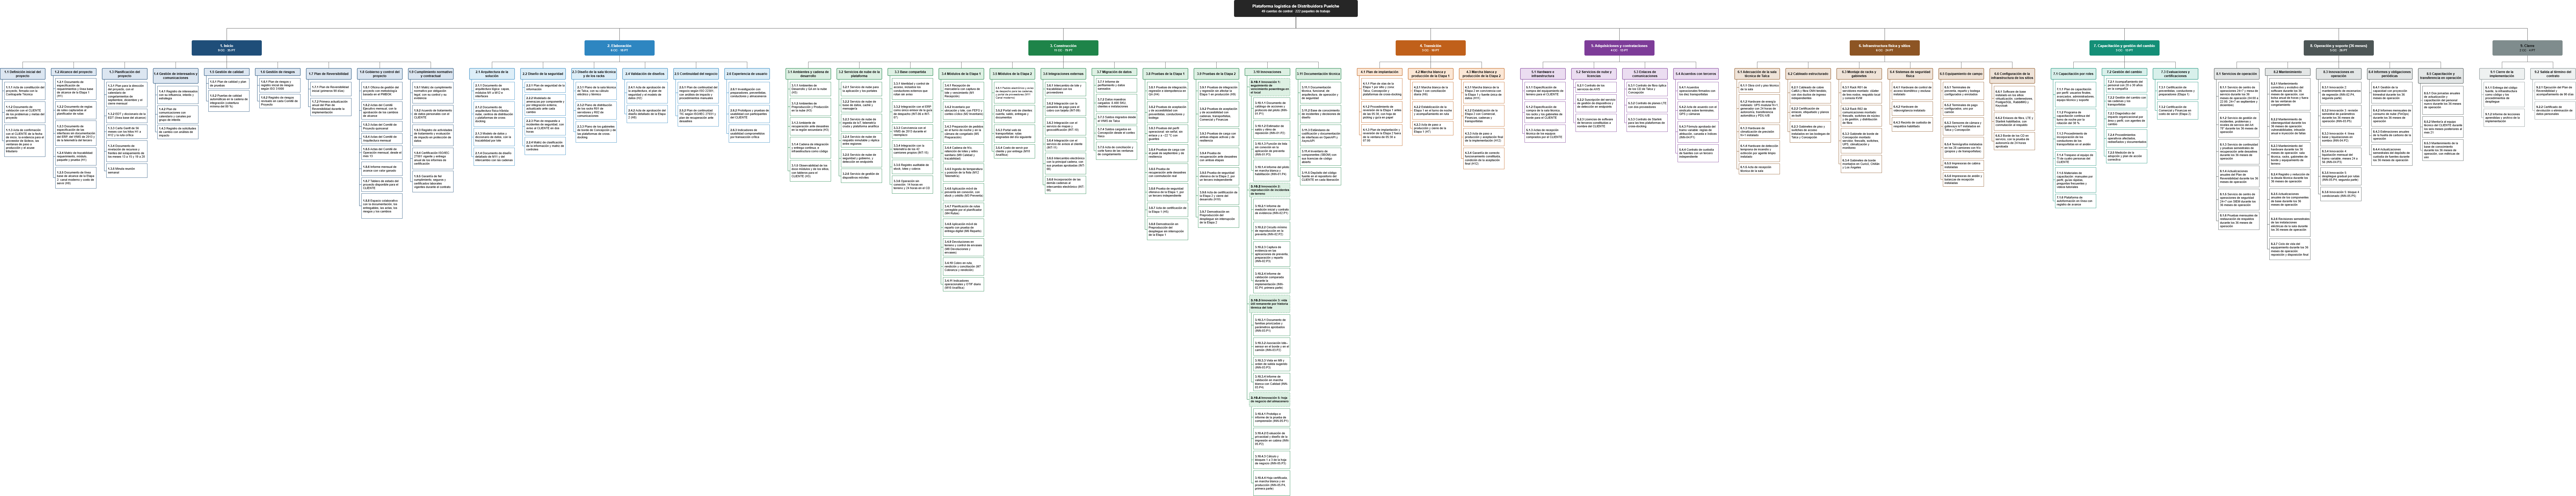
\includegraphics[width=0.98\linewidth,keepaspectratio]{imagenes/Imagenes de la edt/EDT completa.drawio.png}
  \captionsetup{hypcap=false}
  \captionof{figure}{Vista panorámica de la EDT completa del proyecto. Para consultar el detalle por fase, véanse las láminas de la sección «Estructura general» del Subdocumento 7. Fuente: elaboración propia a partir del Formulario T-14.}
  \label{fig:T14-edt-completa}
\end{center}
\end{anexohorizontal}

\section{Diccionario de la EDT}

El diccionario describe cada paquete con su entregable, su criterio de aceptación, su responsable y el período del cronograma en que se ejecuta, con el hito del Formulario E-25 que habilita cuando corresponde. Todo entregable se recibe con un acta de la Contraparte Técnica (Bases Administrativas, Art. 18.1), que acompaña la evidencia de verificación, la trazabilidad hacia los requerimientos del Formulario T-12 y las observaciones resueltas (Art. 18.2). Los criterios de cada paquete se suman a esa regla común.

Los responsables son los roles de la estructura para el proyecto del Capítulo 1, sección 1.5. La Tabla \ref{tab:T14-2} presenta las siglas usadas en el diccionario.

\parte{tablas/tab_T14_2}

Los paquetes de la fase 8 son paquetes de esfuerzo continuo. Cada uno cubre un servicio durante los 36 meses de operación y se controla con entregables mensuales o anuales, como el informe de servicio, el informe de pruebas o la actualización de un plan; esos entregables son sus puntos de verificación.

\subsection{Fase 1. Inicio}

La fase 1 reúne 9 cuentas de control y 35 paquetes de trabajo.

\subsubsection{Cuenta 1.1 — Definición inicial del proyecto}

Esta cuenta de control reúne los tres documentos con que el proyecto arranca formalmente.

La Tabla \ref{tab:T-14-3} presenta sus paquetes.

\parte{tablas/tab_T14_3}

\subsubsection{Cuenta 1.2 — Alcance del proyecto}

Esta cuenta de control fija qué se construye y deja todo listo para diseñar. Incluye la captura del conocimiento del planificador y el levantamiento de las interfaces, porque ambos son insumos del alcance.

La Tabla \ref{tab:T-14-4} presenta sus paquetes.

\parte{tablas/tab_T14_4}

\subsubsection{Cuenta 1.3 — Planificación del proyecto}

Esta cuenta de control reúne los documentos que dicen cómo y cuándo se hará el trabajo, y los informes que muestran si se cumple.

La Tabla \ref{tab:T-14-5} presenta sus paquetes.

\parte{tablas/tab_T14_5}

\subsubsection{Cuenta 1.4 — Gestión de interesados y comunicaciones}

Esta cuenta de control reúne el trabajo con las personas que pueden apoyar o frenar el proyecto, y el lugar donde se toman las decisiones.

La Tabla \ref{tab:T-14-6} presenta sus paquetes.

\parte{tablas/tab_T14_6}

\subsubsection{Cuenta 1.5 — Gestión de calidad}

Esta cuenta de control reúne las reglas que impiden que algo defectuoso llegue a los usuarios.

La Tabla \ref{tab:T-14-7} presenta sus paquetes.

\parte{tablas/tab_T14_7}

\subsubsection{Cuenta 1.6 — Gestión de riesgos}

Esta cuenta de control mantiene vivo el registro de riesgos y verifica que cada respuesta se ejecute.

La Tabla \ref{tab:T-14-8} presenta sus paquetes.

\parte{tablas/tab_T14_8}

\subsubsection{Cuenta 1.7 — Plan de Reversibilidad}

Esta cuenta de control asegura que Puelche pueda cambiar de proveedor o asumir la operación sin interrumpir el servicio. Lo exige el Art. 77°.

La Tabla \ref{tab:T-14-9} presenta sus paquetes.

\parte{tablas/tab_T14_9}

\subsubsection{Cuenta 1.8 — Gobierno y control del proyecto}

Esta cuenta de control reúne las instancias de gobierno que el Art. 71° de las Bases Administrativas hace obligatorias para ambas partes, y los mecanismos de control y reporte del capítulo 19 de las Bases Técnicas Transversales. Las actas de todos los comités se levantan dentro de los dos días hábiles siguientes, con acuerdos, responsables y plazos (RT-19.09).

La Tabla \ref{tab:T-14-10} presenta sus paquetes.

\parte{tablas/tab_T14_10}

\subsubsection{Cuenta 1.9 — Cumplimiento normativo y contractual}

Esta cuenta de control reúne las obligaciones legales y contractuales que no producen software, pero que el contrato exige mantener y acreditar: cumplimiento normativo, datos personales, certificación de seguridad, garantías, seguros y obligaciones laborales.

La Tabla \ref{tab:T-14-11} presenta sus paquetes.

\parte{tablas/tab_T14_11}

\subsection{Fase 2. Elaboración}

La fase 2 reúne 6 cuentas de control y 18 paquetes de trabajo.

\subsubsection{Cuenta 2.1 — Arquitectura de la solución}

Esta cuenta de control reúne los planos técnicos del software y de su emplazamiento.

La Tabla \ref{tab:T-14-12} presenta sus paquetes.

\parte{tablas/tab_T14_12}

\subsubsection{Cuenta 2.2 — Diseño de la seguridad}

Esta cuenta de control define cómo se protegen los datos y los accesos.

La Tabla \ref{tab:T-14-13} presenta sus paquetes.

\parte{tablas/tab_T14_13}

\subsubsection{Cuenta 2.3 — Diseño de la sala técnica y de los racks}

Esta cuenta de control reúne los planos de la infraestructura física que se instala en la fase 6. La sala actual de Talca tiene 25 m², un aire acondicionado de pared y una UPS que dura 10 minutos, y no cumple el estándar exigido (Caso, cap. 5 y 16).

La Tabla \ref{tab:T-14-14} presenta sus paquetes.

\parte{tablas/tab_T14_14}

\subsubsection{Cuenta 2.4 — Validación de diseños}

Esta cuenta de control reúne las dos actas que cierran las fases de Elaboración y dan acceso a los hitos de pago.

La Tabla \ref{tab:T-14-15} presenta sus paquetes.

\parte{tablas/tab_T14_15}

\subsubsection{Cuenta 2.5 — Continuidad del negocio}

Esta cuenta de control reúne los planes que dicen cómo sigue operando Puelche si la solución, un sitio o un proveedor fallan. Va más allá de la recuperación técnica (3.1.3): incluye contingencias auxiliares manuales cuando el proceso las admite. El despacho de 96 camiones entre 05:30 y 07:00 requiere continuidad tecnológica probada, sin sustitución manual ni interrupción.

La Tabla \ref{tab:T-14-16} presenta sus paquetes.

\parte{tablas/tab_T14_16}

\subsubsection{Cuenta 2.6 — Experiencia de usuario}

Esta cuenta de control reúne el trabajo de diseñar la solución con las personas que la van a usar, \textbf{antes} de construirla. Lo exige el Art. 26°. En Puelche es decisivo: preparadores con guantes a −22 °C, preventistas sin señal, conductores externos que se incorporan en minutos y almaceneros sin internet.

La Tabla \ref{tab:T-14-17} presenta sus paquetes.

\parte{tablas/tab_T14_17}

\subsection{Fase 3. Construcción}

La fase 3 reúne 11 cuentas de control y 79 paquetes de trabajo.

\subsubsection{Cuenta 3.1 — Ambientes y cadena de desarrollo}

Esta cuenta de control reúne los lugares donde el software se construye, se prueba y se ejecuta, y las herramientas que lo mueven entre ellos. Las Bases exigen cinco ambientes: Desarrollo, QA, Preproducción, Producción y Recuperación ante desastres.

La Tabla \ref{tab:T-14-18} presenta sus paquetes.

\parte{tablas/tab_T14_18}

\subsubsection{Cuenta 3.2 — Servicios de nube de la plataforma}

Esta cuenta de control reúne la puesta en marcha de cada servicio de nube del T-11, antes de que el software lo use. Contratar el servicio no basta: hay que configurarlo según el plan de seguridad y conectarlo a la observabilidad.

La Tabla \ref{tab:T-14-19} presenta sus paquetes.

\parte{tablas/tab_T14_19}

\subsubsection{Cuenta 3.3 — Base compartida}

Esta cuenta de control reúne los servicios de software que usan los doce módulos. Se construyen primero porque, si fallan, fallan todos los módulos a la vez.

La Tabla \ref{tab:T-14-20} presenta sus paquetes.

\parte{tablas/tab_T14_20}

\subsubsection{Cuenta 3.4 — Módulos de la Etapa 1}

Esta cuenta de control reúne los once programas que la Etapa 1 pone en producción en el mes 16. Cada uno es un paquete. Se construye por iteraciones de RUP y entra al H4 (mes 10) con QA superado.

La Tabla \ref{tab:T-14-21} presenta sus paquetes.

\parte{tablas/tab_T14_21}

\subsubsection{Cuenta 3.5 — Módulos de la Etapa 2}

Esta cuenta de control reúne lo que la Etapa 2 pone en producción en el mes 21. Se construye entre los meses 13 y 18, mientras la Etapa 1 está en marcha blanca. Entra al H9 (mes 17) con QA superado.

La Tabla \ref{tab:T-14-22} presenta sus paquetes.

\parte{tablas/tab_T14_22}

\subsubsection{Cuenta 3.6 — Integraciones externas}

Esta cuenta de control reúne las conexiones con terceros que no están en la base compartida. Llevan el código de interfaz de la arquitectura del Capítulo 4. Cada integración tiene una conducta definida para cuando el tercero falla, para que una caída externa no detenga la operación.

La Tabla \ref{tab:T-14-23} presenta sus paquetes.

\parte{tablas/tab_T14_23}

\subsubsection{Cuenta 3.7 — Migración de datos}

Esta cuenta de control reúne el traslado de los datos actuales a la nueva solución. Las Bases exigen dos ensayos antes de la migración definitiva y una conciliación sin diferencias no explicadas (Bases Técnicas Transversales, numeral 20.1).

La Tabla \ref{tab:T-14-24} presenta sus paquetes.

\parte{tablas/tab_T14_24}

\subsubsection{Cuenta 3.8 — Pruebas de la Etapa 1}

Esta cuenta de control reúne las pruebas que exigen las Bases antes del paso a producción de la Etapa 1, y el acta que las certifica. Cada prueba tiene su criterio de salida en el Bases Técnicas Transversales, numeral 20.1.

La Tabla \ref{tab:T-14-25} presenta sus paquetes.

\parte{tablas/tab_T14_25}

\subsubsection{Cuenta 3.9 — Pruebas de la Etapa 2}

Esta cuenta de control reúne las mismas pruebas para la Etapa 2, con una exigencia adicional: demostrar que la Etapa 1, ya en producción, no se degrada.

La Tabla \ref{tab:T-14-26} presenta sus paquetes.

\parte{tablas/tab_T14_26}

\subsubsection{Cuenta 3.10 — Innovaciones}

Esta cuenta de control reúne los paquetes de construcción de las innovaciones 1, 2, 3 y 5. La parte de la innovación 4 que se hace antes de la Operación está en la fase 5 (5.4.3), porque es un diseño contractual. Las partes que ocurren durante la Operación están en la fase 8. Las metas son propuestas de diseño.

La Tabla \ref{tab:T-14-27} presenta sus paquetes.

\parte{tablas/tab_T14_27}

\subsubsection{Cuenta 3.11 — Documentación técnica}

Esta cuenta de control reúne lo que permite entender, mantener y traspasar la solución. Lo exige el Art. 77°.

La Tabla \ref{tab:T-14-28} presenta sus paquetes.

\parte{tablas/tab_T14_28}

\subsection{Fase 4. Transición}

La fase 4 reúne 3 cuentas de control y 10 paquetes de trabajo.

\subsubsection{Cuenta 4.1 — Plan de implantación}

Esta cuenta de control reúne los planes que dicen cómo entra la solución y cómo se vuelve atrás si algo falla.

La Tabla \ref{tab:T-14-29} presenta sus paquetes.

\parte{tablas/tab_T14_29}

\subsubsection{Cuenta 4.2 — Marcha blanca y producción de la Etapa 1}

Esta cuenta de control reúne la operación supervisada de la Etapa 1, el acompañamiento posterior y el acta que la convierte en el registro oficial.

La Tabla \ref{tab:T-14-30} presenta sus paquetes.

\parte{tablas/tab_T14_30}

\subsubsection{Cuenta 4.3 — Marcha blanca y producción de la Etapa 2}

Esta cuenta de control es igual a la 4.2, aplicada a la Etapa 2. Agrega una condición: convivir con la Etapa 1 ya en producción, con una sola fuente de verdad para los datos compartidos.

La Tabla \ref{tab:T-14-31} presenta sus paquetes.

\parte{tablas/tab_T14_31}

\subsection{Fase 5. Adquisiciones y contrataciones}

La fase 5 reúne 4 cuentas de control y 13 paquetes de trabajo.

\subsubsection{Cuenta 5.1 — Hardware e infraestructura}

Esta cuenta de control reúne la especificación del equipamiento de terreno que compra el CLIENTE, la especificación y compra de la infraestructura que provee LafroX y su recepción técnica. LafroX provee, instala, integra y mantiene la infraestructura dentro del precio del contrato (Bases Administrativas, art. 14.2), con valorización en la Oferta Económica (art. 50.2).

La Tabla \ref{tab:T-14-32} presenta sus paquetes.

\parte{tablas/tab_T14_32}

\subsubsection{Cuenta 5.2 — Servicios de nube y licencias}

Esta cuenta de control reúne los servicios de software que LafroX contrata.

La Tabla \ref{tab:T-14-33} presenta sus paquetes.

\parte{tablas/tab_T14_33}

\subsubsection{Cuenta 5.3 — Enlaces de comunicaciones}

Esta cuenta de control reúne los contratos de conexión de los sitios que contrata LafroX. El caso nombra la dependencia de un solo enlace en Concepción como un riesgo, y Los Ángeles tiene señal intermitente justo en su ventana de madrugada. Cada CD tiene fibra como enlace principal, LTE de respaldo y Starlink como tercer camino en espera caliente. Cada plataforma de cross-docking tiene Starlink como enlace principal y LTE de dos proveedores como respaldo.

La Tabla \ref{tab:T-14-34} presenta sus paquetes.

\parte{tablas/tab_T14_34}

\subsubsection{Cuenta 5.4 — Acuerdos con terceros}

Esta cuenta de control reúne los acuerdos sin los cuales la solución no puede salir a la ruta, y la fórmula contractual de la innovación 4.

La Tabla \ref{tab:T-14-35} presenta sus paquetes.

\parte{tablas/tab_T14_35}

\subsection{Fase 6. Infraestructura física y sitios}

La fase 6 reúne 6 cuentas de control y 24 paquetes de trabajo.

\subsubsection{Cuenta 6.1 — Adecuación de la sala técnica de Talca}

Esta cuenta de control reúne el trabajo de convertir la sala de Talca en una sala técnica que cumpla las Bases (BTT, capítulo 6). Termina con un acta que habilita el montaje de los racks.

La Tabla \ref{tab:T-14-36} presenta sus paquetes.

\parte{tablas/tab_T14_36}

\subsubsection{Cuenta 6.2 — Cableado estructurado}

Esta cuenta de control reúne la red física de cables que conecta los equipos de la sala y de las bodegas.

La Tabla \ref{tab:T-14-37} presenta sus paquetes.

\parte{tablas/tab_T14_37}

\subsubsection{Cuenta 6.3 — Montaje de racks y gabinetes}

Esta cuenta de control reúne el montaje de los equipos de cómputo y comunicaciones en cada uno de los cinco sitios.

La Tabla \ref{tab:T-14-38} presenta sus paquetes.

\parte{tablas/tab_T14_38}

\subsubsection{Cuenta 6.4 — Sistemas de seguridad física}

Esta cuenta de control reúne lo que protege físicamente a la sala y a sus respaldos.

La Tabla \ref{tab:T-14-39} presenta sus paquetes.

\parte{tablas/tab_T14_39}

\subsubsection{Cuenta 6.5 — Equipamiento de campo}

Esta cuenta de control reúne la puesta en marcha de los equipos que usan las personas en la bodega y en la ruta. Se instalan por olas, antes de que cada ola empiece.

La Tabla \ref{tab:T-14-40} presenta sus paquetes.

\parte{tablas/tab_T14_40}

\subsubsection{Cuenta 6.6 — Configuración de la infraestructura de los sitios}

Esta cuenta de control reúne lo necesario para que el hardware instalado funcione como plataforma: el software de base, los enlaces y la prueba de autonomía.

La Tabla \ref{tab:T-14-41} presenta sus paquetes.

\parte{tablas/tab_T14_41}

\subsection{Fase 7. Capacitación y gestión del cambio}

La fase 7 reúne 3 cuentas de control y 13 paquetes de trabajo.

\subsubsection{Cuenta 7.1 — Capacitación por roles}

Esta cuenta de control reúne la capacitación de cada grupo según su rol y su situación.

La Tabla \ref{tab:T-14-42} presenta sus paquetes.

\parte{tablas/tab_T14_42}

\subsubsection{Cuenta 7.2 — Gestión del cambio}

Esta cuenta de control reúne el acompañamiento de quienes no basta con capacitar.

La Tabla \ref{tab:T-14-43} presenta sus paquetes.

\parte{tablas/tab_T14_43}

\subsubsection{Cuenta 7.3 — Evaluaciones y certificaciones}

Esta cuenta de control reúne las pruebas con que se demuestra que cada persona sabe usar la solución. Es una de las seis condiciones del Art. 17.3.

La Tabla \ref{tab:T-14-44} presenta sus paquetes.

\parte{tablas/tab_T14_44}

\subsection{Fase 8. Operación y soporte (36 meses)}

La fase 8 reúne 5 cuentas de control y 26 paquetes de trabajo.

\subsubsection{Cuenta 8.1 — Servicios de operación}

Esta cuenta de control reúne los servicios que mantienen la solución funcionando cada día y la actualización anual del Plan de Reversibilidad, que exige el Art. 77°.

La Tabla \ref{tab:T-14-45} presenta sus paquetes.

\parte{tablas/tab_T14_45}

\subsubsection{Cuenta 8.2 — Mantenimiento}

Esta cuenta de control reúne el trabajo que mantiene la solución sana y actualizada, separado por tipo: software, ciberseguridad y hardware.

La Tabla \ref{tab:T-14-46} presenta sus paquetes.

\parte{tablas/tab_T14_46}

\subsubsection{Cuenta 8.3 — Innovaciones en operación}

Esta cuenta de control reúne la parte de las innovaciones que ocurre después del mes 21. Las metas son propuestas de diseño.

La Tabla \ref{tab:T-14-47} presenta sus paquetes.

\parte{tablas/tab_T14_47}

\subsubsection{Cuenta 8.4 — Informes y obligaciones periódicas}

Esta cuenta de control reúne los informes y las tareas que las Bases fijan con una periodicidad durante la Operación y que no forman parte de los servicios diarios.

La Tabla \ref{tab:T-14-48} presenta sus paquetes.

\parte{tablas/tab_T14_48}

\subsubsection{Cuenta 8.5 — Capacitación y transferencia en operación}

Esta cuenta de control reúne la capacitación y el traspaso de conocimiento que las Bases exigen después de la implementación.

La Tabla \ref{tab:T-14-49} presenta sus paquetes.

\parte{tablas/tab_T14_49}

\subsection{Fase 9. Cierre}

La fase 9 reúne 2 cuentas de control y 4 paquetes de trabajo.

\subsubsection{Cuenta 9.1 — Cierre de la implementación}

Esta cuenta de control reúne lo que se entrega cuando termina la implementación.

La Tabla \ref{tab:T-14-50} presenta sus paquetes.

\parte{tablas/tab_T14_50}

\subsubsection{Cuenta 9.2 — Salida al término del contrato}

Esta cuenta de control reúne el traspaso final y la eliminación de los datos personales.

La Tabla \ref{tab:T-14-51} presenta sus paquetes.

\parte{tablas/tab_T14_51}

\section{Carta Gantt de 56 meses}

La carta Gantt cubre los 56 meses del contrato y muestra las ventanas de marcha blanca, los pasos a producción y el inicio de la fase de Operación, como exige el Formulario T-14. Su estructura contractual la fija el Art. 17° de las Bases Administrativas, y los hitos y sus meses, el Formulario E-25. La Tabla \ref{tab:T14-gantt} presenta esa estructura fija, sobre la cual se programan los paquetes de la sección 2.

\parte{tablas/tab_T14_52}

Ningún paso a producción, inicio de ola, corte de datos ni intervención con impacto en la facturación o en el inventario valorizado se programa en septiembre, en diciembre ni en los tres primeros días hábiles de un mes (Caso 02, secciones 13.2 y 13.3). La correspondencia entre meses contractuales y meses calendario depende de la fecha de inicio del contrato; se analiza en la sección 7.3.2 del Subdocumento 7 y en su Anexo 7.A, que adoptan como supuesto un inicio en febrero de 2027. La Figura \ref{fig:T14-56} presenta la carta de los 56 meses por período contractual y por fase.

\begin{figure}[htbp]
\LFXfiguraPendiente
\nota{Descripción textual de figura: Periodos del Art. 17° e hitos del E-25 hito mensual Fases de la EDT Marcha blanca Continua o a demanda Septiembre y diciembre (sin pasos a producción) Hito del Formulario E-25}
\caption{Carta Gantt de los 56 meses por período contractual y por fase, con inicio en febrero de 2027. Fuente: elaboración propia a partir de las Bases Administrativas, Art. 17°, del Formulario E-25 y de la sección 2 de este formulario.}
\label{fig:T14-56}
\end{figure}

La carta confirma que los períodos fijos del Art. 17° se cumplen mes a mes y que ningún paso a producción cae en una columna de congelamiento. La sección 3.1 detalla la programación por cuenta de control.

Según la carta de la sección 3.1, la sala técnica y el borde de los sitios se instalan entre los meses 3 y 5, la base compartida y los módulos de la Etapa 1 se construyen entre los meses 5 y 8, y las pruebas de integración y certificación de la Etapa 1 ocupan los meses 9 y 10, antes del H5 del mes 12. Las cuentas de la Etapa 2 (3.5, 3.9, 4.3 y la segunda parte de 5.4) se ubican entre los meses 13 y 22, con los módulos en el mes 15 y la integración y certificación en los meses 16 y 17. Las cuentas de capacitación y de gestión del cambio se intensifican desde el mes 10, en preparación de cada marcha blanca.

\subsection{Carta Gantt por cuenta de control}

La carta siguiente reemplaza como fuente vigente a las figuras anteriores, que conservan la programación previa a la reconciliación de ventanas. Cada barra va desde el primer mes del primer paquete de la cuenta hasta el último mes del último paquete, según la programación por paquete del Formulario T-15 (secciones 4.2 y 6.1); los hitos se ubican al cierre de su mes, salvo H6 y H11, que marcan el inicio de una marcha blanca. El detalle por paquete, con sus 222 ventanas, está en esa misma sección, y la red con revisiones del CLIENTE y ruta crítica, en su sección 5. Las cuentas recurrentes (1.4, 1.8, 1.9, 7.1 y 8) se muestran como barras continuas, aunque su trabajo se ejecute con la frecuencia que fija este diccionario.

\begin{anexohorizontal}
\setlength{\textwidth}{\linewidth}
\begin{center}
\begin{tikzpicture}[x=0.245cm,y=0.36cm,font=\small]
\node[anchor=west,font=\bfseries] at (-30,1) {Carta Gantt vigente: cuentas de control e hitos (1/3)};
\node[font=\tiny] at (0.5,0.35) {1};
\node[font=\tiny] at (1.5,0.35) {2};
\node[font=\tiny] at (2.5,0.35) {3};
\node[font=\tiny] at (3.5,0.35) {4};
\node[font=\tiny] at (4.5,0.35) {5};
\node[font=\tiny] at (5.5,0.35) {6};
\node[font=\tiny] at (6.5,0.35) {7};
\node[font=\tiny] at (7.5,0.35) {8};
\node[font=\tiny] at (8.5,0.35) {9};
\node[font=\tiny] at (9.5,0.35) {10};
\node[font=\tiny] at (10.5,0.35) {11};
\node[font=\tiny] at (11.5,0.35) {12};
\node[font=\tiny] at (12.5,0.35) {13};
\node[font=\tiny] at (13.5,0.35) {14};
\node[font=\tiny] at (14.5,0.35) {15};
\node[font=\tiny] at (15.5,0.35) {16};
\node[font=\tiny] at (16.5,0.35) {17};
\node[font=\tiny] at (17.5,0.35) {18};
\node[font=\tiny] at (18.5,0.35) {19};
\node[font=\tiny] at (19.5,0.35) {20};
\node[font=\tiny] at (20.5,0.35) {21};
\node[font=\tiny] at (21.5,0.35) {22};
\node[font=\tiny] at (22.5,0.35) {23};
\node[font=\tiny] at (23.5,0.35) {24};
\node[font=\tiny] at (24.5,0.35) {25};
\node[font=\tiny] at (25.5,0.35) {26};
\node[font=\tiny] at (26.5,0.35) {27};
\node[font=\tiny] at (27.5,0.35) {28};
\node[font=\tiny] at (28.5,0.35) {29};
\node[font=\tiny] at (29.5,0.35) {30};
\node[font=\tiny] at (30.5,0.35) {31};
\node[font=\tiny] at (31.5,0.35) {32};
\node[font=\tiny] at (32.5,0.35) {33};
\node[font=\tiny] at (33.5,0.35) {34};
\node[font=\tiny] at (34.5,0.35) {35};
\node[font=\tiny] at (35.5,0.35) {36};
\node[font=\tiny] at (36.5,0.35) {37};
\node[font=\tiny] at (37.5,0.35) {38};
\node[font=\tiny] at (38.5,0.35) {39};
\node[font=\tiny] at (39.5,0.35) {40};
\node[font=\tiny] at (40.5,0.35) {41};
\node[font=\tiny] at (41.5,0.35) {42};
\node[font=\tiny] at (42.5,0.35) {43};
\node[font=\tiny] at (43.5,0.35) {44};
\node[font=\tiny] at (44.5,0.35) {45};
\node[font=\tiny] at (45.5,0.35) {46};
\node[font=\tiny] at (46.5,0.35) {47};
\node[font=\tiny] at (47.5,0.35) {48};
\node[font=\tiny] at (48.5,0.35) {49};
\node[font=\tiny] at (49.5,0.35) {50};
\node[font=\tiny] at (50.5,0.35) {51};
\node[font=\tiny] at (51.5,0.35) {52};
\node[font=\tiny] at (52.5,0.35) {53};
\node[font=\tiny] at (53.5,0.35) {54};
\node[font=\tiny] at (54.5,0.35) {55};
\node[font=\tiny] at (55.5,0.35) {56};
\node[anchor=west,font=\bfseries] at (-30,-1) {Hitos E-25};
\node[anchor=west,font=\scriptsize] at (-30,-2) {H1 mes 2};
\fill[lafroxFuerte] (1.82,-2) -- (2,-1.82) -- (2.18,-2) -- (2,-2.18) -- cycle;
\node[anchor=west,font=\scriptsize] at (-30,-3) {H2 mes 4};
\fill[lafroxFuerte] (3.82,-3) -- (4,-2.82) -- (4.18,-3) -- (4,-3.18) -- cycle;
\node[anchor=west,font=\scriptsize] at (-30,-4) {H3 mes 6};
\fill[lafroxFuerte] (5.82,-4) -- (6,-3.82) -- (6.18,-4) -- (6,-4.18) -- cycle;
\node[anchor=west,font=\scriptsize] at (-30,-5) {H4 mes 10};
\fill[lafroxFuerte] (9.82,-5) -- (10,-4.82) -- (10.18,-5) -- (10,-5.18) -- cycle;
\node[anchor=west,font=\scriptsize] at (-30,-6) {H5 mes 12};
\fill[lafroxFuerte] (11.82,-6) -- (12,-5.82) -- (12.18,-6) -- (12,-6.18) -- cycle;
\node[anchor=west,font=\scriptsize] at (-30,-7) {H6 mes 13};
\fill[lafroxFuerte] (11.82,-7) -- (12,-6.82) -- (12.18,-7) -- (12,-7.18) -- cycle;
\node[anchor=west,font=\scriptsize] at (-30,-8) {H8 mes 14};
\fill[lafroxFuerte] (13.82,-8) -- (14,-7.82) -- (14.18,-8) -- (14,-8.18) -- cycle;
\node[anchor=west,font=\scriptsize] at (-30,-9) {H7 mes 16};
\fill[lafroxFuerte] (15.82,-9) -- (16,-8.82) -- (16.18,-9) -- (16,-9.18) -- cycle;
\node[anchor=west,font=\scriptsize] at (-30,-10) {H9 mes 17};
\fill[lafroxFuerte] (16.82,-10) -- (17,-9.82) -- (17.18,-10) -- (17,-10.18) -- cycle;
\node[anchor=west,font=\scriptsize] at (-30,-11) {H10 mes 18};
\fill[lafroxFuerte] (17.82,-11) -- (18,-10.82) -- (18.18,-11) -- (18,-11.18) -- cycle;
\node[anchor=west,font=\scriptsize] at (-30,-12) {H11 mes 19};
\fill[lafroxFuerte] (17.82,-12) -- (18,-11.82) -- (18.18,-12) -- (18,-12.18) -- cycle;
\node[anchor=west,font=\scriptsize] at (-30,-13) {H12 mes 21};
\fill[lafroxFuerte] (20.82,-13) -- (21,-12.82) -- (21.18,-13) -- (21,-13.18) -- cycle;
\node[anchor=west,font=\bfseries] at (-30,-14) {Fase 1 Inicio};
\node[anchor=west,font=\scriptsize] at (-30,-15) {1.1 Definición inicial del proyecto};
\fill[lafroxFuerte!65] (0,-15.23) rectangle (1,-14.77);
\node[anchor=west,font=\scriptsize] at (-30,-16) {1.2 Alcance del proyecto};
\fill[lafroxFuerte!65] (0,-16.23) rectangle (13,-15.77);
\node[anchor=west,font=\scriptsize] at (-30,-17) {1.3 Planificación del proyecto};
\fill[lafroxFuerte!65] (0,-17.23) rectangle (20,-16.77);
\node[anchor=west,font=\scriptsize] at (-30,-18) {1.4 Gestión de interesados y comunicaciones};
\fill[lafroxFuerte!65] (0,-18.23) rectangle (56,-17.77);
\node[anchor=west,font=\scriptsize] at (-30,-19) {1.5 Gestión de calidad};
\fill[lafroxFuerte!65] (1,-19.23) rectangle (20,-18.77);
\node[anchor=west,font=\scriptsize] at (-30,-20) {1.6 Gestión de riesgos};
\fill[lafroxFuerte!65] (0,-20.23) rectangle (20,-19.77);
\node[anchor=west,font=\scriptsize] at (-30,-21) {1.7 Plan de Reversibilidad};
\fill[lafroxFuerte!65] (2,-21.23) rectangle (15,-20.77);
\node[anchor=west,font=\scriptsize] at (-30,-22) {1.8 Gobierno y control del proyecto};
\fill[lafroxFuerte!65] (0,-22.23) rectangle (56,-21.77);
\node[anchor=west,font=\scriptsize] at (-30,-23) {1.9 Cumplimiento normativo y contractual};
\fill[lafroxFuerte!65] (0,-23.23) rectangle (56,-22.77);
\node[anchor=west,font=\bfseries] at (-30,-24) {Fase 2 Elaboración};
\node[anchor=west,font=\scriptsize] at (-30,-25) {2.1 Arquitectura de la solución};
\fill[lafroxFuerte!65] (1,-25.23) rectangle (13,-24.77);
\node[anchor=west,font=\scriptsize] at (-30,-26) {2.2 Diseño de la seguridad};
\fill[lafroxFuerte!65] (1,-26.23) rectangle (10,-25.77);
\node[anchor=west,font=\scriptsize] at (-30,-27) {2.3 Diseño de la sala técnica y de los racks};
\fill[lafroxFuerte!65] (0,-27.23) rectangle (2,-26.77);
\node[anchor=west,font=\scriptsize] at (-30,-28) {2.4 Validación de diseños};
\fill[lafroxFuerte!65] (2,-28.23) rectangle (14,-27.77);
\node[anchor=west,font=\scriptsize] at (-30,-29) {2.5 Continuidad del negocio};
\fill[lafroxFuerte!65] (2,-29.23) rectangle (3,-28.77);
\node[anchor=west,font=\scriptsize] at (-30,-30) {2.6 Experiencia de usuario};
\fill[lafroxFuerte!65] (1,-30.23) rectangle (4,-29.77);
\draw[lafroxGris!20] (0,0) -- (0,-30.6);
\draw[lafroxGris!20] (1,0) -- (1,-30.6);
\draw[lafroxGris!20] (2,0) -- (2,-30.6);
\draw[lafroxGris!20] (3,0) -- (3,-30.6);
\draw[lafroxGris!20] (4,0) -- (4,-30.6);
\draw[lafroxGris!20] (5,0) -- (5,-30.6);
\draw[lafroxGris!20] (6,0) -- (6,-30.6);
\draw[lafroxGris!20] (7,0) -- (7,-30.6);
\draw[lafroxGris!20] (8,0) -- (8,-30.6);
\draw[lafroxGris!20] (9,0) -- (9,-30.6);
\draw[lafroxGris!20] (10,0) -- (10,-30.6);
\draw[lafroxGris!20] (11,0) -- (11,-30.6);
\draw[lafroxGris!20] (12,0) -- (12,-30.6);
\draw[lafroxGris!20] (13,0) -- (13,-30.6);
\draw[lafroxGris!20] (14,0) -- (14,-30.6);
\draw[lafroxGris!20] (15,0) -- (15,-30.6);
\draw[lafroxGris!20] (16,0) -- (16,-30.6);
\draw[lafroxGris!20] (17,0) -- (17,-30.6);
\draw[lafroxGris!20] (18,0) -- (18,-30.6);
\draw[lafroxGris!20] (19,0) -- (19,-30.6);
\draw[lafroxGris!20] (20,0) -- (20,-30.6);
\draw[lafroxGris!20] (21,0) -- (21,-30.6);
\draw[lafroxGris!20] (22,0) -- (22,-30.6);
\draw[lafroxGris!20] (23,0) -- (23,-30.6);
\draw[lafroxGris!20] (24,0) -- (24,-30.6);
\draw[lafroxGris!20] (25,0) -- (25,-30.6);
\draw[lafroxGris!20] (26,0) -- (26,-30.6);
\draw[lafroxGris!20] (27,0) -- (27,-30.6);
\draw[lafroxGris!20] (28,0) -- (28,-30.6);
\draw[lafroxGris!20] (29,0) -- (29,-30.6);
\draw[lafroxGris!20] (30,0) -- (30,-30.6);
\draw[lafroxGris!20] (31,0) -- (31,-30.6);
\draw[lafroxGris!20] (32,0) -- (32,-30.6);
\draw[lafroxGris!20] (33,0) -- (33,-30.6);
\draw[lafroxGris!20] (34,0) -- (34,-30.6);
\draw[lafroxGris!20] (35,0) -- (35,-30.6);
\draw[lafroxGris!20] (36,0) -- (36,-30.6);
\draw[lafroxGris!20] (37,0) -- (37,-30.6);
\draw[lafroxGris!20] (38,0) -- (38,-30.6);
\draw[lafroxGris!20] (39,0) -- (39,-30.6);
\draw[lafroxGris!20] (40,0) -- (40,-30.6);
\draw[lafroxGris!20] (41,0) -- (41,-30.6);
\draw[lafroxGris!20] (42,0) -- (42,-30.6);
\draw[lafroxGris!20] (43,0) -- (43,-30.6);
\draw[lafroxGris!20] (44,0) -- (44,-30.6);
\draw[lafroxGris!20] (45,0) -- (45,-30.6);
\draw[lafroxGris!20] (46,0) -- (46,-30.6);
\draw[lafroxGris!20] (47,0) -- (47,-30.6);
\draw[lafroxGris!20] (48,0) -- (48,-30.6);
\draw[lafroxGris!20] (49,0) -- (49,-30.6);
\draw[lafroxGris!20] (50,0) -- (50,-30.6);
\draw[lafroxGris!20] (51,0) -- (51,-30.6);
\draw[lafroxGris!20] (52,0) -- (52,-30.6);
\draw[lafroxGris!20] (53,0) -- (53,-30.6);
\draw[lafroxGris!20] (54,0) -- (54,-30.6);
\draw[lafroxGris!20] (55,0) -- (55,-30.6);
\draw[lafroxGris!20] (56,0) -- (56,-30.6);
\end{tikzpicture}
\captionsetup{hypcap=false}
\captionof{figure}{Carta Gantt vigente por cuenta de control, parte 1 de 3. Fuente: Formulario T-14 y cronograma del Formulario T-15.}\label{fig:T14-gantt-vigente}
\end{center}
\end{anexohorizontal}

\begin{anexohorizontal}
\setlength{\textwidth}{\linewidth}
\begin{center}
\begin{tikzpicture}[x=0.245cm,y=0.36cm,font=\small]
\node[anchor=west,font=\bfseries] at (-30,1) {Carta Gantt vigente: cuentas de control e hitos (2/3)};
\node[font=\tiny] at (0.5,0.35) {1};
\node[font=\tiny] at (1.5,0.35) {2};
\node[font=\tiny] at (2.5,0.35) {3};
\node[font=\tiny] at (3.5,0.35) {4};
\node[font=\tiny] at (4.5,0.35) {5};
\node[font=\tiny] at (5.5,0.35) {6};
\node[font=\tiny] at (6.5,0.35) {7};
\node[font=\tiny] at (7.5,0.35) {8};
\node[font=\tiny] at (8.5,0.35) {9};
\node[font=\tiny] at (9.5,0.35) {10};
\node[font=\tiny] at (10.5,0.35) {11};
\node[font=\tiny] at (11.5,0.35) {12};
\node[font=\tiny] at (12.5,0.35) {13};
\node[font=\tiny] at (13.5,0.35) {14};
\node[font=\tiny] at (14.5,0.35) {15};
\node[font=\tiny] at (15.5,0.35) {16};
\node[font=\tiny] at (16.5,0.35) {17};
\node[font=\tiny] at (17.5,0.35) {18};
\node[font=\tiny] at (18.5,0.35) {19};
\node[font=\tiny] at (19.5,0.35) {20};
\node[font=\tiny] at (20.5,0.35) {21};
\node[font=\tiny] at (21.5,0.35) {22};
\node[font=\tiny] at (22.5,0.35) {23};
\node[font=\tiny] at (23.5,0.35) {24};
\node[font=\tiny] at (24.5,0.35) {25};
\node[font=\tiny] at (25.5,0.35) {26};
\node[font=\tiny] at (26.5,0.35) {27};
\node[font=\tiny] at (27.5,0.35) {28};
\node[font=\tiny] at (28.5,0.35) {29};
\node[font=\tiny] at (29.5,0.35) {30};
\node[font=\tiny] at (30.5,0.35) {31};
\node[font=\tiny] at (31.5,0.35) {32};
\node[font=\tiny] at (32.5,0.35) {33};
\node[font=\tiny] at (33.5,0.35) {34};
\node[font=\tiny] at (34.5,0.35) {35};
\node[font=\tiny] at (35.5,0.35) {36};
\node[font=\tiny] at (36.5,0.35) {37};
\node[font=\tiny] at (37.5,0.35) {38};
\node[font=\tiny] at (38.5,0.35) {39};
\node[font=\tiny] at (39.5,0.35) {40};
\node[font=\tiny] at (40.5,0.35) {41};
\node[font=\tiny] at (41.5,0.35) {42};
\node[font=\tiny] at (42.5,0.35) {43};
\node[font=\tiny] at (43.5,0.35) {44};
\node[font=\tiny] at (44.5,0.35) {45};
\node[font=\tiny] at (45.5,0.35) {46};
\node[font=\tiny] at (46.5,0.35) {47};
\node[font=\tiny] at (47.5,0.35) {48};
\node[font=\tiny] at (48.5,0.35) {49};
\node[font=\tiny] at (49.5,0.35) {50};
\node[font=\tiny] at (50.5,0.35) {51};
\node[font=\tiny] at (51.5,0.35) {52};
\node[font=\tiny] at (52.5,0.35) {53};
\node[font=\tiny] at (53.5,0.35) {54};
\node[font=\tiny] at (54.5,0.35) {55};
\node[font=\tiny] at (55.5,0.35) {56};
\node[anchor=west,font=\bfseries] at (-30,-1) {Fase 3 Construcción};
\node[anchor=west,font=\scriptsize] at (-30,-2) {3.1 Ambientes y cadena de desarrollo};
\fill[lafroxFuerte!65] (3,-2.23) rectangle (5,-1.77);
\node[anchor=west,font=\scriptsize] at (-30,-3) {3.2 Servicios de nube de la plataforma};
\fill[lafroxFuerte!65] (3,-3.23) rectangle (5,-2.77);
\node[anchor=west,font=\scriptsize] at (-30,-4) {3.3 Base compartida};
\fill[lafroxFuerte!65] (4,-4.23) rectangle (7,-3.77);
\node[anchor=west,font=\scriptsize] at (-30,-5) {3.4 Módulos de la Etapa 1};
\fill[lafroxFuerte!65] (4,-5.23) rectangle (8,-4.77);
\node[anchor=west,font=\scriptsize] at (-30,-6) {3.5 Módulos de la Etapa 2};
\fill[lafroxFuerte!65] (14,-6.23) rectangle (15,-5.77);
\node[anchor=west,font=\scriptsize] at (-30,-7) {3.6 Integraciones externas};
\fill[lafroxFuerte!65] (6,-7.23) rectangle (19,-6.77);
\node[anchor=west,font=\scriptsize] at (-30,-8) {3.7 Migración de datos};
\fill[lafroxFuerte!65] (6,-8.23) rectangle (12,-7.77);
\node[anchor=west,font=\scriptsize] at (-30,-9) {3.8 Pruebas de la Etapa 1};
\fill[lafroxFuerte!65] (8,-9.23) rectangle (10,-8.77);
\node[anchor=west,font=\scriptsize] at (-30,-10) {3.9 Pruebas de la Etapa 2};
\fill[lafroxFuerte!65] (15,-10.23) rectangle (17,-9.77);
\node[anchor=west,font=\scriptsize] at (-30,-11) {3.10 Innovaciones};
\fill[lafroxFuerte!65] (1,-11.23) rectangle (21,-10.77);
\node[anchor=west,font=\scriptsize] at (-30,-12) {3.11 Documentación técnica};
\fill[lafroxFuerte!65] (3,-12.23) rectangle (21,-11.77);
\node[anchor=west,font=\bfseries] at (-30,-13) {Fase 4 Transición};
\node[anchor=west,font=\scriptsize] at (-30,-14) {4.1 Plan de implantación};
\fill[lafroxFuerte!65] (9,-14.23) rectangle (17,-13.77);
\node[anchor=west,font=\scriptsize] at (-30,-15) {4.2 Marcha blanca y producción de la Etapa 1};
\fill[lafroxFuerte!65] (12,-15.23) rectangle (20,-14.77);
\node[anchor=west,font=\scriptsize] at (-30,-16) {4.3 Marcha blanca y producción de la Etapa 2};
\fill[lafroxFuerte!65] (18,-16.23) rectangle (22,-15.77);
\node[anchor=west,font=\bfseries] at (-30,-17) {Fase 5 Adquisiciones y contrataciones};
\node[anchor=west,font=\scriptsize] at (-30,-18) {5.1 Hardware e infraestructura};
\fill[lafroxFuerte!65] (1,-18.23) rectangle (5,-17.77);
\node[anchor=west,font=\scriptsize] at (-30,-19) {5.2 Servicios de nube y licencias};
\fill[lafroxFuerte!65] (1,-19.23) rectangle (4,-18.77);
\node[anchor=west,font=\scriptsize] at (-30,-20) {5.3 Enlaces de comunicaciones};
\fill[lafroxFuerte!65] (3,-20.23) rectangle (4,-19.77);
\node[anchor=west,font=\scriptsize] at (-30,-21) {5.4 Acuerdos con terceros};
\fill[lafroxFuerte!65] (6,-21.23) rectangle (20,-20.77);
\draw[lafroxGris!20] (0,0) -- (0,-21.6);
\draw[lafroxGris!20] (1,0) -- (1,-21.6);
\draw[lafroxGris!20] (2,0) -- (2,-21.6);
\draw[lafroxGris!20] (3,0) -- (3,-21.6);
\draw[lafroxGris!20] (4,0) -- (4,-21.6);
\draw[lafroxGris!20] (5,0) -- (5,-21.6);
\draw[lafroxGris!20] (6,0) -- (6,-21.6);
\draw[lafroxGris!20] (7,0) -- (7,-21.6);
\draw[lafroxGris!20] (8,0) -- (8,-21.6);
\draw[lafroxGris!20] (9,0) -- (9,-21.6);
\draw[lafroxGris!20] (10,0) -- (10,-21.6);
\draw[lafroxGris!20] (11,0) -- (11,-21.6);
\draw[lafroxGris!20] (12,0) -- (12,-21.6);
\draw[lafroxGris!20] (13,0) -- (13,-21.6);
\draw[lafroxGris!20] (14,0) -- (14,-21.6);
\draw[lafroxGris!20] (15,0) -- (15,-21.6);
\draw[lafroxGris!20] (16,0) -- (16,-21.6);
\draw[lafroxGris!20] (17,0) -- (17,-21.6);
\draw[lafroxGris!20] (18,0) -- (18,-21.6);
\draw[lafroxGris!20] (19,0) -- (19,-21.6);
\draw[lafroxGris!20] (20,0) -- (20,-21.6);
\draw[lafroxGris!20] (21,0) -- (21,-21.6);
\draw[lafroxGris!20] (22,0) -- (22,-21.6);
\draw[lafroxGris!20] (23,0) -- (23,-21.6);
\draw[lafroxGris!20] (24,0) -- (24,-21.6);
\draw[lafroxGris!20] (25,0) -- (25,-21.6);
\draw[lafroxGris!20] (26,0) -- (26,-21.6);
\draw[lafroxGris!20] (27,0) -- (27,-21.6);
\draw[lafroxGris!20] (28,0) -- (28,-21.6);
\draw[lafroxGris!20] (29,0) -- (29,-21.6);
\draw[lafroxGris!20] (30,0) -- (30,-21.6);
\draw[lafroxGris!20] (31,0) -- (31,-21.6);
\draw[lafroxGris!20] (32,0) -- (32,-21.6);
\draw[lafroxGris!20] (33,0) -- (33,-21.6);
\draw[lafroxGris!20] (34,0) -- (34,-21.6);
\draw[lafroxGris!20] (35,0) -- (35,-21.6);
\draw[lafroxGris!20] (36,0) -- (36,-21.6);
\draw[lafroxGris!20] (37,0) -- (37,-21.6);
\draw[lafroxGris!20] (38,0) -- (38,-21.6);
\draw[lafroxGris!20] (39,0) -- (39,-21.6);
\draw[lafroxGris!20] (40,0) -- (40,-21.6);
\draw[lafroxGris!20] (41,0) -- (41,-21.6);
\draw[lafroxGris!20] (42,0) -- (42,-21.6);
\draw[lafroxGris!20] (43,0) -- (43,-21.6);
\draw[lafroxGris!20] (44,0) -- (44,-21.6);
\draw[lafroxGris!20] (45,0) -- (45,-21.6);
\draw[lafroxGris!20] (46,0) -- (46,-21.6);
\draw[lafroxGris!20] (47,0) -- (47,-21.6);
\draw[lafroxGris!20] (48,0) -- (48,-21.6);
\draw[lafroxGris!20] (49,0) -- (49,-21.6);
\draw[lafroxGris!20] (50,0) -- (50,-21.6);
\draw[lafroxGris!20] (51,0) -- (51,-21.6);
\draw[lafroxGris!20] (52,0) -- (52,-21.6);
\draw[lafroxGris!20] (53,0) -- (53,-21.6);
\draw[lafroxGris!20] (54,0) -- (54,-21.6);
\draw[lafroxGris!20] (55,0) -- (55,-21.6);
\draw[lafroxGris!20] (56,0) -- (56,-21.6);
\end{tikzpicture}
\captionsetup{hypcap=false}
\captionof{figure}{Carta Gantt vigente por cuenta de control, parte 2 de 3. Fuente: Formulario T-14 y cronograma del Formulario T-15.}
\end{center}
\end{anexohorizontal}

\begin{anexohorizontal}
\setlength{\textwidth}{\linewidth}
\begin{center}
\begin{tikzpicture}[x=0.245cm,y=0.36cm,font=\small]
\node[anchor=west,font=\bfseries] at (-30,1) {Carta Gantt vigente: cuentas de control e hitos (3/3)};
\node[font=\tiny] at (0.5,0.35) {1};
\node[font=\tiny] at (1.5,0.35) {2};
\node[font=\tiny] at (2.5,0.35) {3};
\node[font=\tiny] at (3.5,0.35) {4};
\node[font=\tiny] at (4.5,0.35) {5};
\node[font=\tiny] at (5.5,0.35) {6};
\node[font=\tiny] at (6.5,0.35) {7};
\node[font=\tiny] at (7.5,0.35) {8};
\node[font=\tiny] at (8.5,0.35) {9};
\node[font=\tiny] at (9.5,0.35) {10};
\node[font=\tiny] at (10.5,0.35) {11};
\node[font=\tiny] at (11.5,0.35) {12};
\node[font=\tiny] at (12.5,0.35) {13};
\node[font=\tiny] at (13.5,0.35) {14};
\node[font=\tiny] at (14.5,0.35) {15};
\node[font=\tiny] at (15.5,0.35) {16};
\node[font=\tiny] at (16.5,0.35) {17};
\node[font=\tiny] at (17.5,0.35) {18};
\node[font=\tiny] at (18.5,0.35) {19};
\node[font=\tiny] at (19.5,0.35) {20};
\node[font=\tiny] at (20.5,0.35) {21};
\node[font=\tiny] at (21.5,0.35) {22};
\node[font=\tiny] at (22.5,0.35) {23};
\node[font=\tiny] at (23.5,0.35) {24};
\node[font=\tiny] at (24.5,0.35) {25};
\node[font=\tiny] at (25.5,0.35) {26};
\node[font=\tiny] at (26.5,0.35) {27};
\node[font=\tiny] at (27.5,0.35) {28};
\node[font=\tiny] at (28.5,0.35) {29};
\node[font=\tiny] at (29.5,0.35) {30};
\node[font=\tiny] at (30.5,0.35) {31};
\node[font=\tiny] at (31.5,0.35) {32};
\node[font=\tiny] at (32.5,0.35) {33};
\node[font=\tiny] at (33.5,0.35) {34};
\node[font=\tiny] at (34.5,0.35) {35};
\node[font=\tiny] at (35.5,0.35) {36};
\node[font=\tiny] at (36.5,0.35) {37};
\node[font=\tiny] at (37.5,0.35) {38};
\node[font=\tiny] at (38.5,0.35) {39};
\node[font=\tiny] at (39.5,0.35) {40};
\node[font=\tiny] at (40.5,0.35) {41};
\node[font=\tiny] at (41.5,0.35) {42};
\node[font=\tiny] at (42.5,0.35) {43};
\node[font=\tiny] at (43.5,0.35) {44};
\node[font=\tiny] at (44.5,0.35) {45};
\node[font=\tiny] at (45.5,0.35) {46};
\node[font=\tiny] at (46.5,0.35) {47};
\node[font=\tiny] at (47.5,0.35) {48};
\node[font=\tiny] at (48.5,0.35) {49};
\node[font=\tiny] at (49.5,0.35) {50};
\node[font=\tiny] at (50.5,0.35) {51};
\node[font=\tiny] at (51.5,0.35) {52};
\node[font=\tiny] at (52.5,0.35) {53};
\node[font=\tiny] at (53.5,0.35) {54};
\node[font=\tiny] at (54.5,0.35) {55};
\node[font=\tiny] at (55.5,0.35) {56};
\node[anchor=west,font=\bfseries] at (-30,-1) {Fase 6 Infraestructura física y sitios};
\node[anchor=west,font=\scriptsize] at (-30,-2) {6.1 Adecuación de la sala técnica de Talca};
\fill[lafroxFuerte!65] (2,-2.23) rectangle (4,-1.77);
\node[anchor=west,font=\scriptsize] at (-30,-3) {6.2 Cableado estructurado};
\fill[lafroxFuerte!65] (3,-3.23) rectangle (7,-2.77);
\node[anchor=west,font=\scriptsize] at (-30,-4) {6.3 Montaje de racks y gabinetes};
\fill[lafroxFuerte!65] (3,-4.23) rectangle (9,-3.77);
\node[anchor=west,font=\scriptsize] at (-30,-5) {6.4 Sistemas de seguridad física};
\fill[lafroxFuerte!65] (4,-5.23) rectangle (6,-4.77);
\node[anchor=west,font=\scriptsize] at (-30,-6) {6.5 Equipamiento de campo};
\fill[lafroxFuerte!65] (8,-6.23) rectangle (12,-5.77);
\node[anchor=west,font=\scriptsize] at (-30,-7) {6.6 Configuración de la infraestructura de los sitios};
\fill[lafroxFuerte!65] (4,-7.23) rectangle (5,-6.77);
\node[anchor=west,font=\bfseries] at (-30,-8) {Fase 7 Capacitación y gestión del cambio};
\node[anchor=west,font=\scriptsize] at (-30,-9) {7.1 Capacitación por roles};
\fill[lafroxFuerte!65] (9,-9.23) rectangle (56,-8.77);
\node[anchor=west,font=\scriptsize] at (-30,-10) {7.2 Gestión del cambio};
\fill[lafroxFuerte!65] (1,-10.23) rectangle (21,-9.77);
\node[anchor=west,font=\scriptsize] at (-30,-11) {7.3 Evaluaciones y certificaciones};
\fill[lafroxFuerte!65] (12,-11.23) rectangle (18,-10.77);
\node[anchor=west,font=\bfseries] at (-30,-12) {Fase 8 Operación y soporte};
\node[anchor=west,font=\scriptsize] at (-30,-13) {8.1 Servicios de operación};
\fill[lafroxFuerte!65] (12,-13.23) rectangle (56,-12.77);
\node[anchor=west,font=\scriptsize] at (-30,-14) {8.2 Mantenimiento};
\fill[lafroxFuerte!65] (20,-14.23) rectangle (56,-13.77);
\node[anchor=west,font=\scriptsize] at (-30,-15) {8.3 Innovaciones en operación};
\fill[lafroxFuerte!65] (20,-15.23) rectangle (56,-14.77);
\node[anchor=west,font=\scriptsize] at (-30,-16) {8.4 Informes y obligaciones periódicas};
\fill[lafroxFuerte!65] (20,-16.23) rectangle (56,-15.77);
\node[anchor=west,font=\scriptsize] at (-30,-17) {8.5 Capacitación y transferencia en operación};
\fill[lafroxFuerte!65] (20,-17.23) rectangle (56,-16.77);
\node[anchor=west,font=\bfseries] at (-30,-18) {Fase 9 Cierre};
\node[anchor=west,font=\scriptsize] at (-30,-19) {9.1 Cierre de la implementación};
\fill[lafroxFuerte!65] (20,-19.23) rectangle (21,-18.77);
\node[anchor=west,font=\scriptsize] at (-30,-20) {9.2 Salida al término del contrato};
\fill[lafroxFuerte!65] (53,-20.23) rectangle (56,-19.77);
\draw[lafroxGris!20] (0,0) -- (0,-20.6);
\draw[lafroxGris!20] (1,0) -- (1,-20.6);
\draw[lafroxGris!20] (2,0) -- (2,-20.6);
\draw[lafroxGris!20] (3,0) -- (3,-20.6);
\draw[lafroxGris!20] (4,0) -- (4,-20.6);
\draw[lafroxGris!20] (5,0) -- (5,-20.6);
\draw[lafroxGris!20] (6,0) -- (6,-20.6);
\draw[lafroxGris!20] (7,0) -- (7,-20.6);
\draw[lafroxGris!20] (8,0) -- (8,-20.6);
\draw[lafroxGris!20] (9,0) -- (9,-20.6);
\draw[lafroxGris!20] (10,0) -- (10,-20.6);
\draw[lafroxGris!20] (11,0) -- (11,-20.6);
\draw[lafroxGris!20] (12,0) -- (12,-20.6);
\draw[lafroxGris!20] (13,0) -- (13,-20.6);
\draw[lafroxGris!20] (14,0) -- (14,-20.6);
\draw[lafroxGris!20] (15,0) -- (15,-20.6);
\draw[lafroxGris!20] (16,0) -- (16,-20.6);
\draw[lafroxGris!20] (17,0) -- (17,-20.6);
\draw[lafroxGris!20] (18,0) -- (18,-20.6);
\draw[lafroxGris!20] (19,0) -- (19,-20.6);
\draw[lafroxGris!20] (20,0) -- (20,-20.6);
\draw[lafroxGris!20] (21,0) -- (21,-20.6);
\draw[lafroxGris!20] (22,0) -- (22,-20.6);
\draw[lafroxGris!20] (23,0) -- (23,-20.6);
\draw[lafroxGris!20] (24,0) -- (24,-20.6);
\draw[lafroxGris!20] (25,0) -- (25,-20.6);
\draw[lafroxGris!20] (26,0) -- (26,-20.6);
\draw[lafroxGris!20] (27,0) -- (27,-20.6);
\draw[lafroxGris!20] (28,0) -- (28,-20.6);
\draw[lafroxGris!20] (29,0) -- (29,-20.6);
\draw[lafroxGris!20] (30,0) -- (30,-20.6);
\draw[lafroxGris!20] (31,0) -- (31,-20.6);
\draw[lafroxGris!20] (32,0) -- (32,-20.6);
\draw[lafroxGris!20] (33,0) -- (33,-20.6);
\draw[lafroxGris!20] (34,0) -- (34,-20.6);
\draw[lafroxGris!20] (35,0) -- (35,-20.6);
\draw[lafroxGris!20] (36,0) -- (36,-20.6);
\draw[lafroxGris!20] (37,0) -- (37,-20.6);
\draw[lafroxGris!20] (38,0) -- (38,-20.6);
\draw[lafroxGris!20] (39,0) -- (39,-20.6);
\draw[lafroxGris!20] (40,0) -- (40,-20.6);
\draw[lafroxGris!20] (41,0) -- (41,-20.6);
\draw[lafroxGris!20] (42,0) -- (42,-20.6);
\draw[lafroxGris!20] (43,0) -- (43,-20.6);
\draw[lafroxGris!20] (44,0) -- (44,-20.6);
\draw[lafroxGris!20] (45,0) -- (45,-20.6);
\draw[lafroxGris!20] (46,0) -- (46,-20.6);
\draw[lafroxGris!20] (47,0) -- (47,-20.6);
\draw[lafroxGris!20] (48,0) -- (48,-20.6);
\draw[lafroxGris!20] (49,0) -- (49,-20.6);
\draw[lafroxGris!20] (50,0) -- (50,-20.6);
\draw[lafroxGris!20] (51,0) -- (51,-20.6);
\draw[lafroxGris!20] (52,0) -- (52,-20.6);
\draw[lafroxGris!20] (53,0) -- (53,-20.6);
\draw[lafroxGris!20] (54,0) -- (54,-20.6);
\draw[lafroxGris!20] (55,0) -- (55,-20.6);
\draw[lafroxGris!20] (56,0) -- (56,-20.6);
\end{tikzpicture}
\captionsetup{hypcap=false}
\captionof{figure}{Carta Gantt vigente por cuenta de control, parte 3 de 3. Fuente: Formulario T-14 y cronograma del Formulario T-15.}
\end{center}
\end{anexohorizontal}

\section{Criterios vigentes de programación y recursos}

Las ventanas mensuales de asignación y las HH por paquete están en el T-15, sección 4. La preparación del H3 sigue esta secuencia: planos 2.3.1/\allowbreak{}2.3.2 en el mes 1, especificación y orden de compra de LafroX 5.1.2 en el mes 2, instalación 6.1.1–6.1.4 en el mes 3 y recepción 6.1.5 en el mes 4. Los racks R01/\allowbreak{}R02 se montan en los meses 4 y 5, el gabinete de Concepción en el mes 4 y el borde de los CD entra en servicio mediante 6.6.3 en el mes 5. Los gabinetes de cross-docking se montan en el mes 9. El CLIENTE compra el equipamiento de terreno antes de cada ola.

4.2.2 incorpora estabilización y soporte puente E1 en los meses 16–20, después del paso a producción del H7. La fase contractual de Operación comienza en el mes 21. 4.3.2 comprende cuatro semanas reforzadas posteriores al H12, imputadas a los meses 21 y 22. El T-18, sección 6, declara la dotación y la regla de decremento. 8.3.2 realiza la revisión INN-03.P5 cada seis meses: meses 26, 32, 38, 44, 50 y 56, contados desde el inicio de Operación. El esfuerzo equivalente mensual del T-15 conserva esta frecuencia. La coordinación de reserva y retención (SD4, apartado 4.1.4.4) y las pruebas AL-STOCK-01/\allowbreak{}AL-ACT-01 se incorporan a los paquetes existentes conforme al T-18, sección 6.5. AL-STOCK-01 mide la proporción de líneas con más de una retención y las pruebas de carga 3.8.4/\allowbreak{}3.9.3 verifican el drenaje.

\section{Referencias}

Las Bases se citan con su documento y el artículo, capítulo o sección.

\begin{itemize}
\item Distribuidora Puelche S.A. (2026a). \emph{Bases Administrativas de Licitación N.º TFEP-01/\allowbreak{}2026: Contratación de Solución Integral de Software y Servicios de Operación}.

\item Distribuidora Puelche S.A. (2026c). \emph{Caso 02: Logística. Especificaciones del problema y operación de Distribuidora Puelche S.A.}

\item Distribuidora Puelche S.A. (2026d). \emph{Aclaraciones de la Licitación N.º TFEP-01/\allowbreak{}2026}.

\end{itemize}
\section{Declaración de uso de IA}

En cumplimiento de la sección 7.2 de las Aclaraciones de la licitación, la tabla siguiente declara el uso de herramientas de inteligencia artificial en este formulario, con la revisión humana de cada parte. La declaración se consolida en el Formulario A-6.

\parte{tablas/tab_T14_53}

